\documentclass{llncs}
\usepackage {tikz}
\usepackage{listings}
\usepackage{enumerate}
\usepackage{bibtopic}
\setcounter{tocdepth}{5}
\setcounter{secnumdepth}{5}
\graphicspath{ {./} }
\title{Tehnical Documentation MersulTrenurilor}
\author{Valentin Ro\c sca \\ Grupa B2}
\institute{Faculty of Computer Science of University "Alexandru Ioan Cuza"}
\definecolor{RoyalBlue}{cmyk}{1, 0.50, 0, 0}
\lstset{language=C++,
	keywordstyle=\color{RoyalBlue},
	basicstyle=\scriptsize\ttfamily,
	commentstyle=\ttfamily\itshape\color{gray},
	stringstyle=\ttfamily,
	showstringspaces=false,
	breaklines=true,
	frameround=ffff,
	frame=single,
	rulecolor=\color{black}
} 

\begin{document}
	\maketitle
	\newpage
	
	\begin{abstract}
		This project involves the homework for the Networking class at the Faculty of Computer Science of University "Alexandru Ioan Cuza" and also a solution for the poor train timetable information problems in my country. This paper describes the basic layout of data structures and the process of serving a request and sending it back to the client. This document does not describe any of the algorithms used for different types of requests, only how to server divides it's tasks and code description.
	\end{abstract}

	\section[Introduction]{Introduction}
		\subsection{Overview}
		A server that updates and offers information in real time for all connected clients for:
		\begin{itemize}
			\item arrival status
			\item departures status
			\item delays and arrival estimate
			\item path between stations
		\end{itemize}
	
		\subsection{Purpose}
			\subsubsection{Business Perspective}
				The app offers clients a way to consult train timetables from their home devices like PCs and laptops and to find out the best possible route to take between two cities.
			\subsubsection{Motivation}
				The motivation comes from the possibility to develop my coding skills and distributed algorithms thinking and also from a real need of an application to make the process of staying in touch with train timetables and finding to optimal route effortlessly.
			\subsubsection{Considerations}
				Although the application has read usage in the real world, there are many applications similar and they support a wider range of devices, proving that this is not the perfect solution for all the problems.
		\subsection{Conventions and Abbreviations}
			\subsection{Coding style}
				The coding style used for the C++ source code is the Google C++ Style. For more details, visit the address specified in the references section.
			\subsection{Abbreviations}
				\subsubsection{UML}
					The Unified Modeling Language (UML) is a general-purpose, developmental, modeling language in the field of software engineering, that is intended to provide a standard way to visualize the design of a system.
				\subsubsection{TCP}
					The Transmission Control Protocol (TCP) is one of the main protocols of the Internet protocol suite. It originated in the initial network implementation in which it complemented the Internet Protocol (IP). Therefore, the entire suite is commonly referred to as TCP/IP.
	\section{Technologies and Programming Languages}
		\subsection{Programming Languages}
			\subsection{C++14}
				The main programming language used for the client, server and UI implementation is C++14. The motivation for using this programming language is that it's fast, reliable and comes with a good documentation and support for multi-threading and low-level implementations.
			\subsection{Cypher}
				This is the language used for retrieving and storing the time tables data. This language comes with the nod4j database.
		\subsection{Networking}
			\subsubsection{TCP Sockets}
			For the communication between clients and the server is provided by sockets. The TCP protocol is preferred over UDP because the connection must be kept alive and there shouldn't be any data loss.
		\subsection{UI}
			The user will interact with the application through a graphical user interface (GUI).
			\subsubsection{QT}
				QT is a graphical user interface library that is fast, reliable and comes with a C++ driver.
		\subsection{Databases}
			The data will be kept in a graph structure with stations being the nodes and routes being the edges. This allows to find the shortest path faster than relational models and the data is stored in a natural way for the problem at hand. 
			\subsubsection{Nod4j} 
				Nod4j is a highly scalable, native graph database purpose-build to leverage not only data but also its relationships.
	\section{Application Architecture}
		\subsection{UML}
		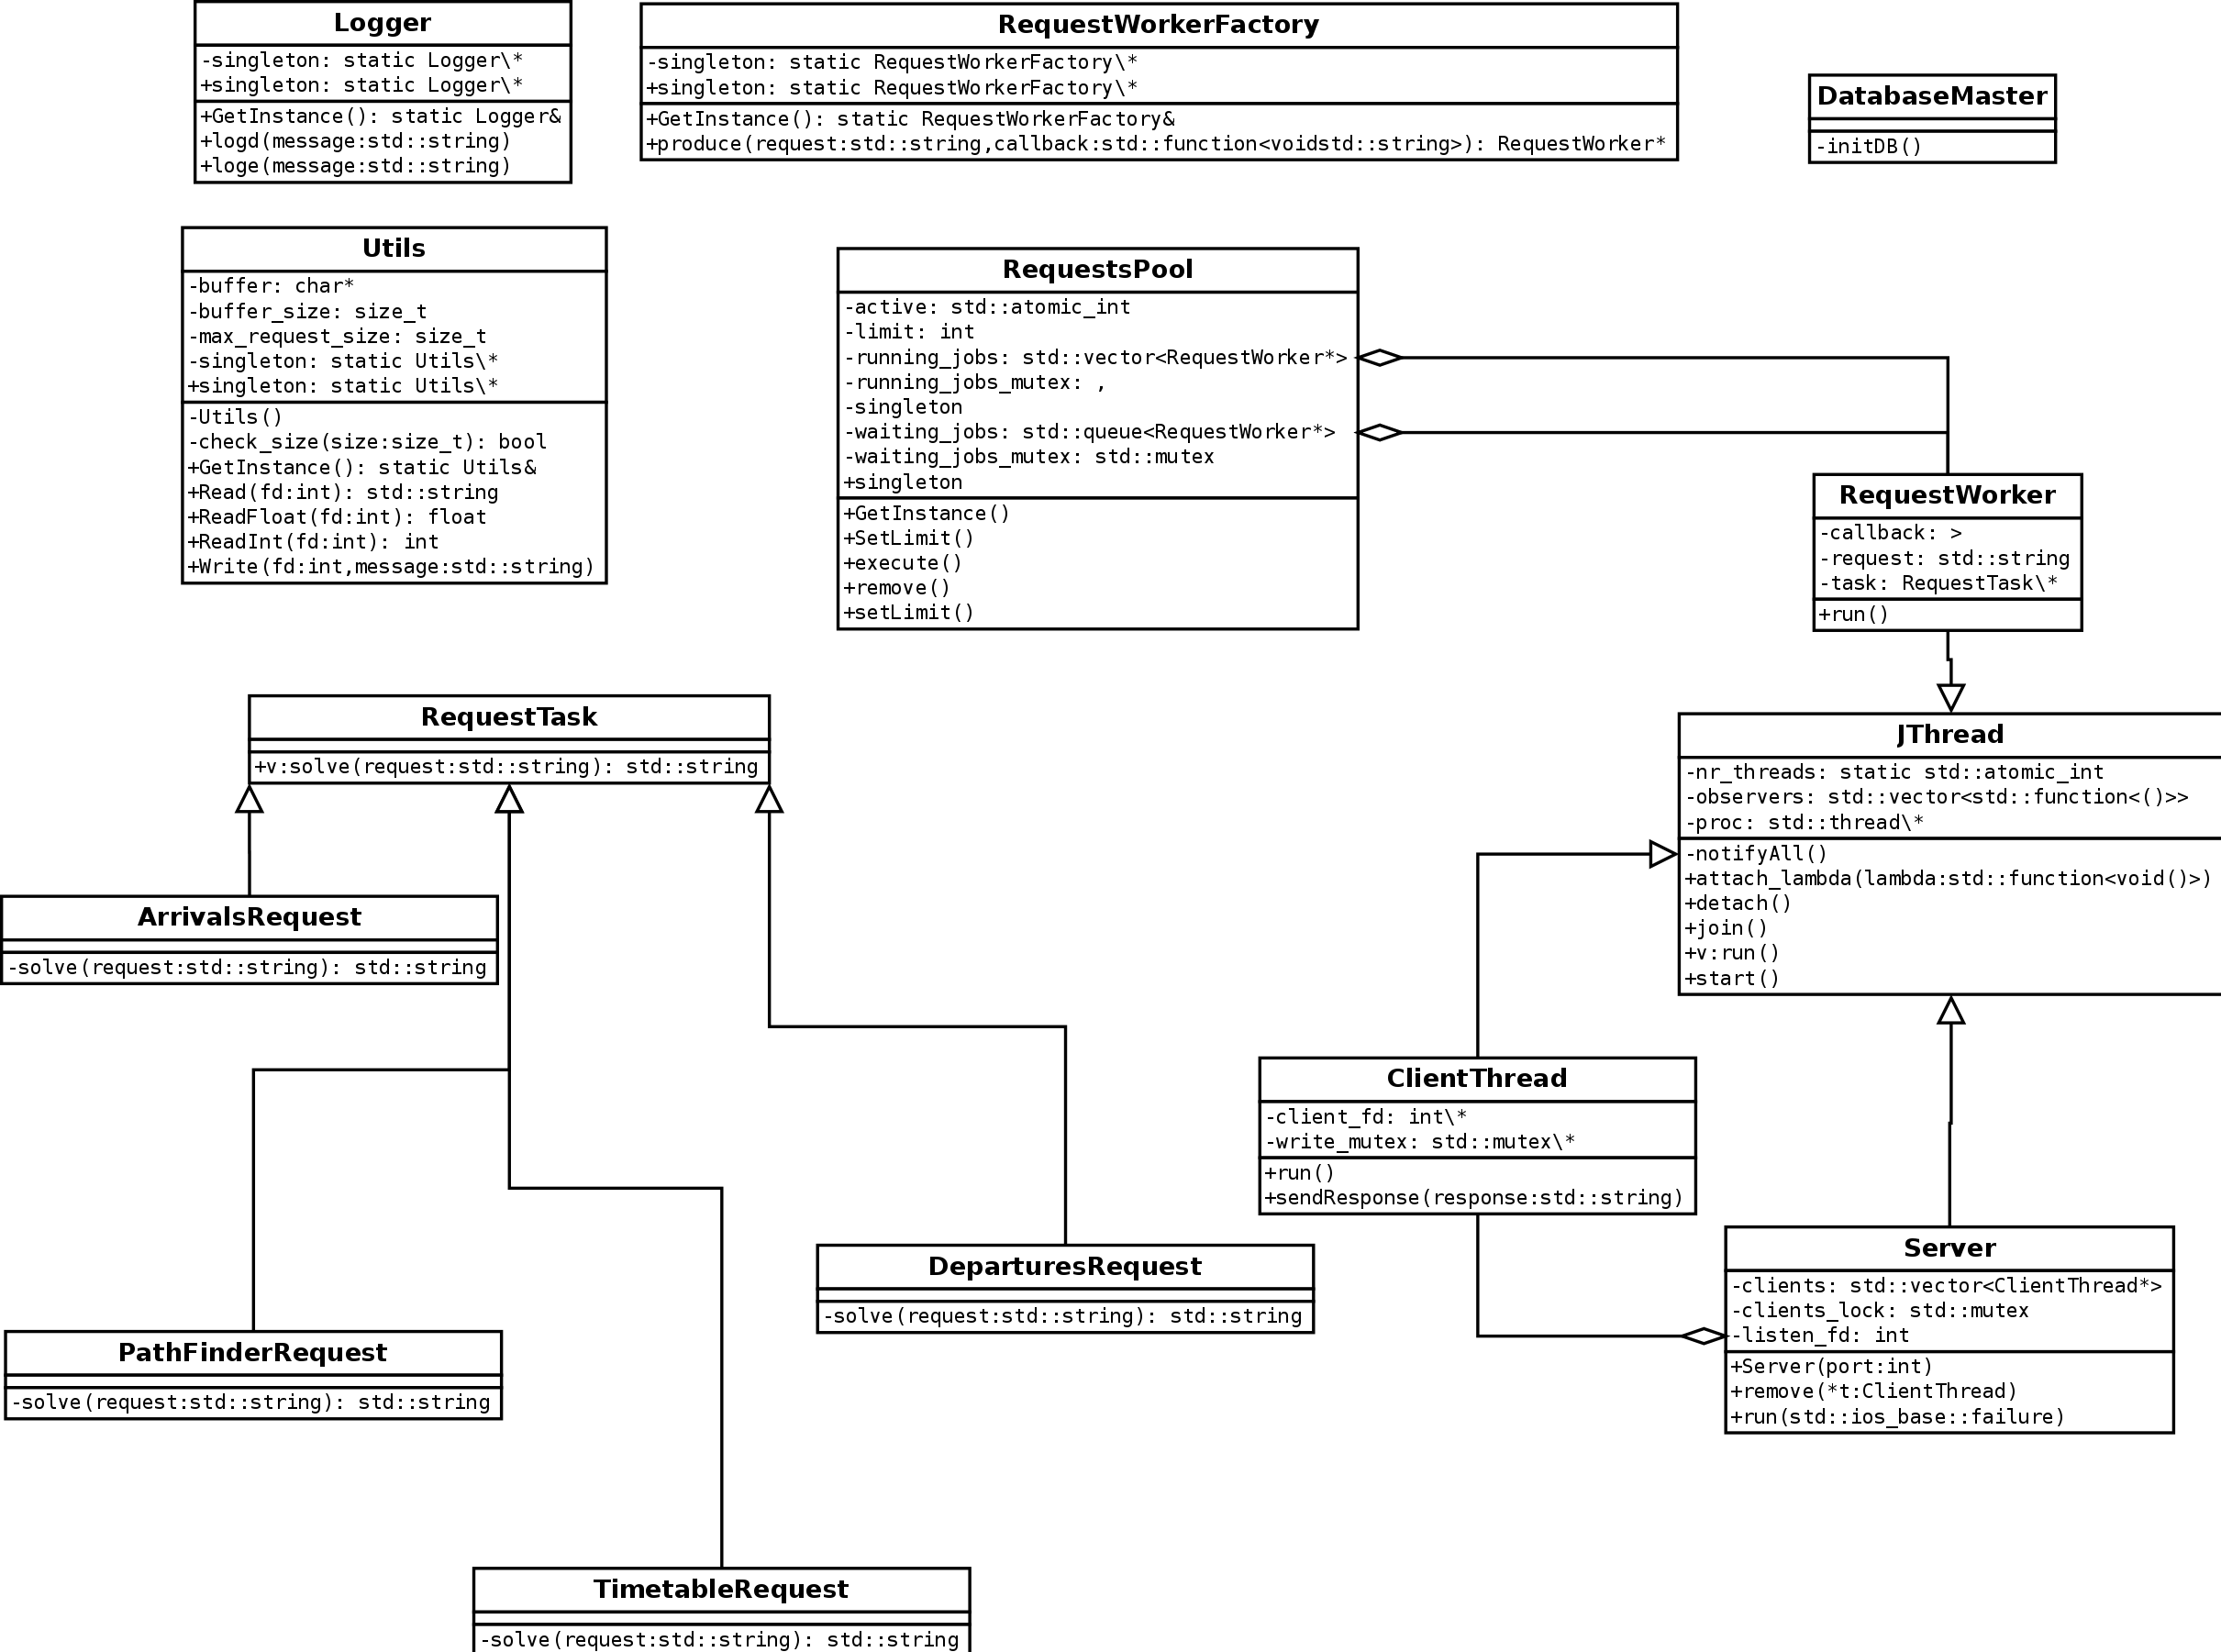
\includegraphics{output}
		\\
		\\
		\\
		\\
		\\
		\\
		\\
		\\
		\\
		\\
		\\
		\\
		\\
		This UML contains the major classes and intefaces for the server side. Because of it's simplicity, the client side does not have an UML diagram.
		\\
		\\
		\\
		\\
		\\
		\\
		\subsection{Diagrama Aplicatiei}
		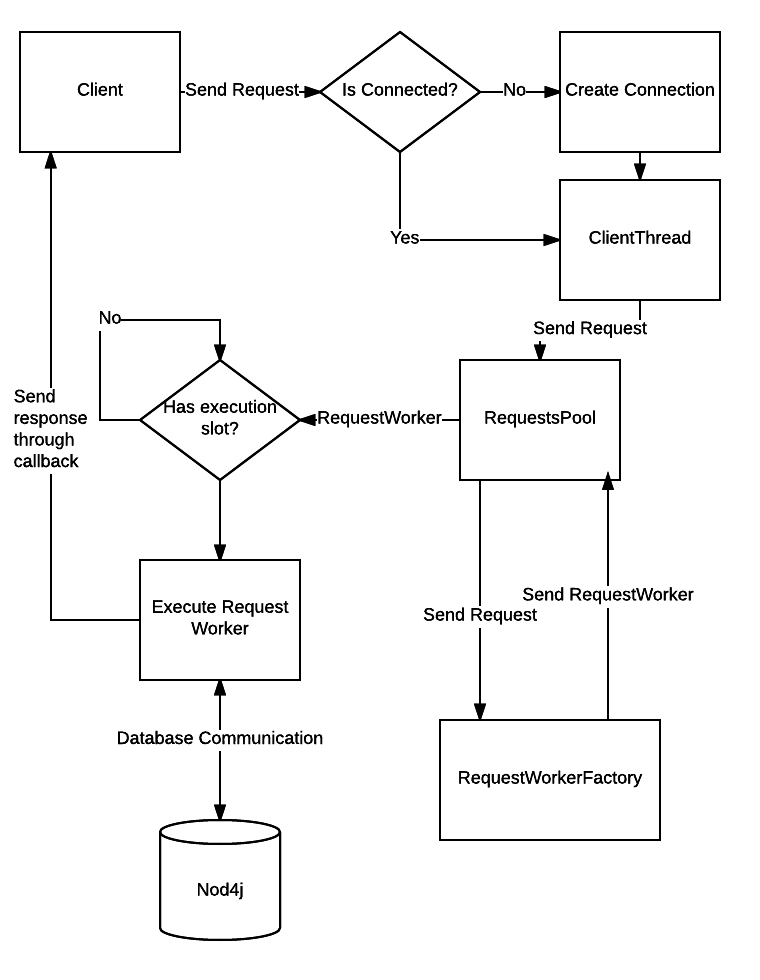
\includegraphics{MersulTrenurilorDiagram}
		\newpage
	\section{Implementation Details}
		\subsection{JThread}
			JThread is a wrapper class for std::thread that allows for easier management and storage through polimorfism of threads. It also supports lambda functions as observers. The notifyAll is called when the run function finishes.
			\begin{lstlisting}
class JThread {
	static std::atomic_int nr_threads;
	std::thread *proc; // the thread object
	void notifyAll (); // notify all observers
public:
	// calls the run function on another thread
	void start (); 				
	void join (); // joins the thread if is joinable				
	void detach (); // detach the thread
					
	// main thread logic - this must me implemented
	// by derivate classes
	virtual void run () = 0;
	
	// attach lambda observer
	void attach_lambda(std::function<void()> lambda);
};
			\end{lstlisting}
			
			
Implementations for the functions above (abstract class JThread):
			\begin{lstlisting}
std::atomic_int JThread::nr_threads{0};
			
void JThread::join () {
	if (proc->joinable())
		proc->join();
}
			
void JThread::start () {
	nr_threads++;
	proc = new std::thread ([this](){run();notifyAll();});
}
			
void JThread::detach () {
	proc->detach();
}
			
void JThread::attach_lambda(std::function<void()> lambda) {
	observers.push_back (lambda);
}
			
void JThread::notifyAll () {
	for (auto i : observers) {
		i();
	}
}
			\end{lstlisting}
			\newpage
		\subsection{Server and ClientThread}
			The Server class extends the JThread class and contains the main server logic. This includes
			\begin{itemize}
				\item socket creation
				\item port binding
				\item listening
				\item creating ClientThreads when a new connection arrives
			\end{itemize}
			
			\begin{lstlisting}
listen(listen_fd, 5);
while (true)
{
	// accept client
	int client_fd = accept(listen_fd, (struct sockaddr *)NULL, NULL);
	Logger::GetInstance().logd("Client accepted. Reading from socket " + std::to_string(client_fd));
			
	if (client_fd < 0)
		throw std::ios_base::failure("Cannot accept client");
			
	// devirate class of JThread controlling the loop that
	// keeps the client connection alive and forwards the requests
	ClientThread client(client_fd);
	clients.push_back (client);
	//remove client when connection is dropped
	client->attach_lambda([this, client]{ this->remove (client);});
	client.start(); // start receiving
}
			\end{lstlisting}
			
			ClientThread is another JThread extension and represents a worker thread that manages a connection with a single client. The purpose of this class is to capture user requests and pass them to the RequestsPool to be solved.
		\subsection{RequestsPool, RequestsWorker and RequestTask}
			RequestsPool uses the command design pattern to solve incoming requests and through callbacks send back the response. This implies that we need to alocate a limited number of workers threads (RequestWorkers extends JThread) with the task at hand and remove them when the execution is finished.
			
Sample for Command Design Pattern job queuing:
			\begin{lstlisting}
worker->attach_lambda([this, worker](){this->remove(worker);});
if (active < limit) { // check for limit of workers 
	worker->run ();
	running_jobs_mutex.lock ();
	running_jobs.push_back (worker);
	running_jobs_mutex.unlock ();
}
else {
	waiting_jobs_mutex.lock ();
	waiting_jobs.push (worker);
	waiting_jobs_mutex.unlock ();
}
			\end{lstlisting}
			\newpage
			
			The RequestTask is an interface for the request types that the user can request. Derivate classes can be found in the UML.
			\begin{lstlisting}
class RequestTask {
public:
	RequestTask() {};
	
	// each derivate class must implement this method 
	// to serve the incoming request
	virtual std::string solve (std::string request) = 0;
};
			\end{lstlisting}
	\section{Conclusions}
	The potential of the project is great but its limitations, the devices it can support and the lack of support for constant database updates can be solved by hiring employees and offer a website for the clients to support multiple devices.
	
	As for the technologies used, I learned to use graph database, integrate them with C++ language and schedule and scheme multi-threaded operations and concurrent access to the database.	
	\begin{thebibliography}{4}
		\bibitem{doc:nod4j} Neo4j - https://neo4j.com/
		\bibitem{doc:latex} Latex Manual - https://en.wikibooks.org/wiki/LaTeX
		\bibitem{doc:C++} C++ Docs - http://www.cplusplus.com/
		\bibitem{doc:wiki} TCP/IP https://en.wikipedia.org/wiki/Transmission\_Control\_Protocol
	\end{thebibliography}
\end{document}